%%%%%%%%%%%%%%%%%%%%%%%%%%%%%%%%%%%%%%%%
%%     Last few slides
%%%%%%%%%%%%%%%%%%%%%%%%%%%%%%%%%%%%%%%%
\section{Wrapup}
\makesubcontentsslides



\begin{frame}
  \begin{block}{Other Important Topics Not Discussed Here}
    \begin{itemize}
      \item Debugging
      \item Arrays
      \item Pointers
      \item Interfacing to C
      \item Tabs versus spaces
    \end{itemize}
  \end{block}
\end{frame}


\begin{frame}
  \begin{block}{Some languages come and go}
    \begin{center}
      
\includegraphics[scale=.7]{pics/lifecycle}
    \end{center}
  \end{block}
\end{frame}

\begin{frame}
  \begin{block}{But with Fortran\dots}
    \begin{center}
      
\includegraphics[scale=.5]{pics/here_forever}
    \end{center}
  \end{block}
\end{frame}

\begin{frame}
  \begin{block}{Because when the USS Enterprise makes her maiden voyage}
    \begin{center}
      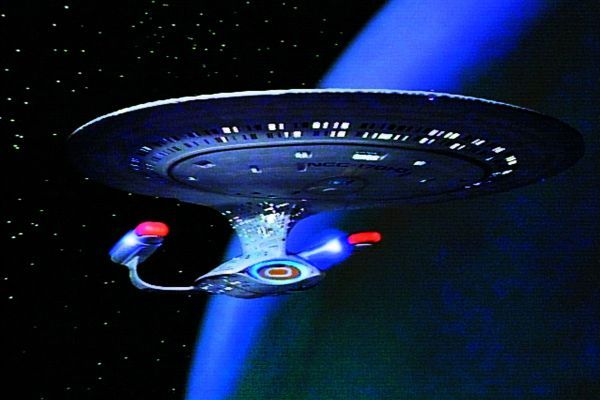
\includegraphics[scale=2]{pics/enterprise}
    \end{center}
  \end{block}
\end{frame}

\begin{frame}
  \begin{block}{Beneath the fancy blinking screens}
    \begin{center}
      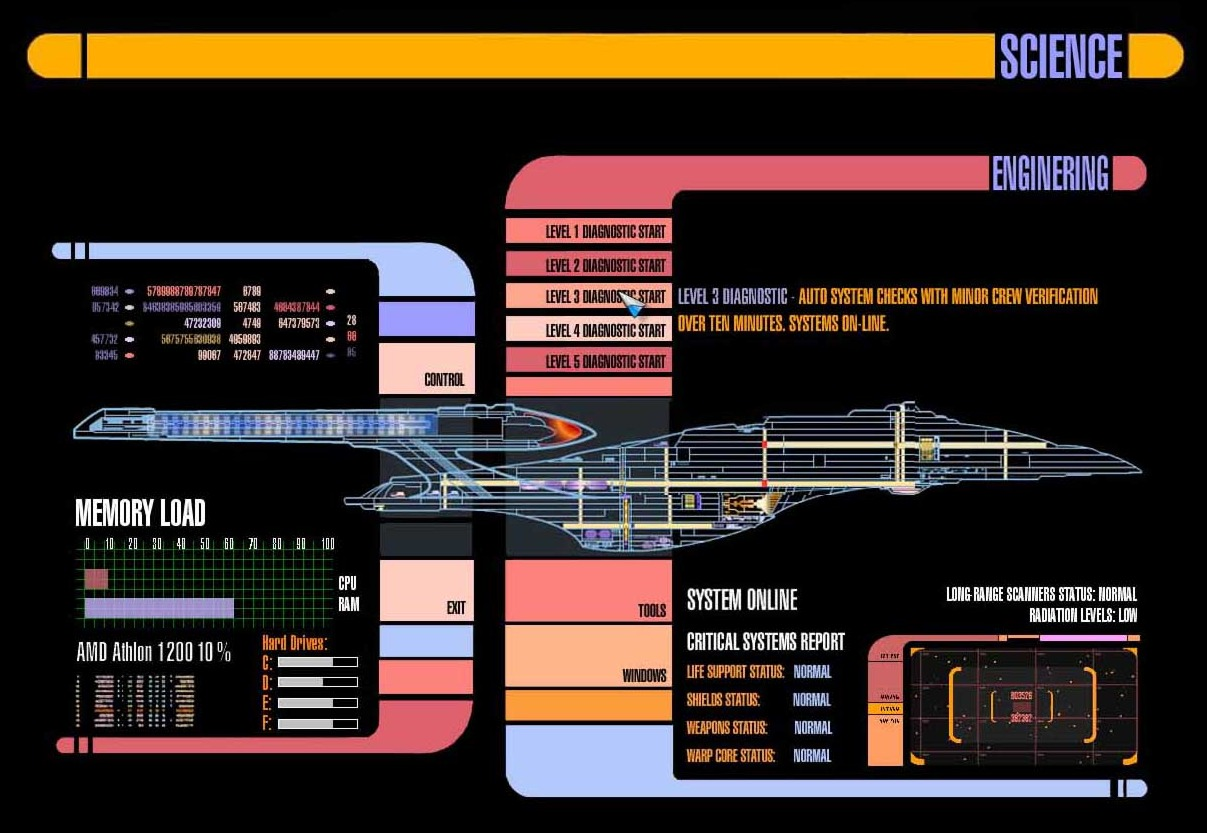
\includegraphics[scale=.33]{pics/lcars}
    \end{center}
  \end{block}
\end{frame}

\begin{frame}
  \begin{block}{You can bet that their crucial systems are powered by Fortran written in the 1970's}
    \begin{center}
      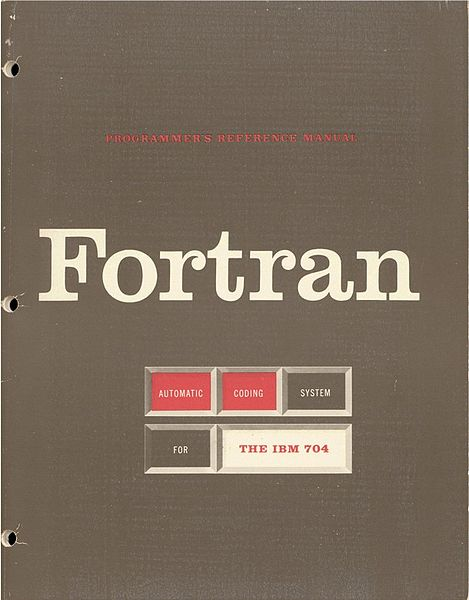
\includegraphics[scale=.3]{pics/fortran}
    \end{center}
  \end{block}
\end{frame}



\section*{}



\begin{frame}[noframenumbering]
 \begin{block}{Thanks for coming!}
 \begin{center}
 \vspace{.4cm}
     {\Huge Questions?}\\[.8cm]
  \end{center}
 \end{block}
\end{frame}
